% Relatório do laboratório 7 de servo
% Felipe Bandeira da Silva
% 20/11/2013

\documentclass[a4paper, 10pt]{article}
%\documentclass[paper=a4, fontsize=11pt]{article}

\usepackage[brazil]{babel}
\usepackage[utf8]{inputenc}
\usepackage{listings}
\usepackage{color}
\usepackage{amsthm}
\usepackage{graphicx}

\usepackage{schemabloc}
\usetikzlibrary{circuits}

\setlength{\parindent}{0pt}
\setlength{\parskip}{18pt}

\title{Relatório, Laboratório 7.\\Servo 1}
\author{Felipe Bandeira da Silva}
\date{}


\begin{document}

\maketitle

Objetivo: Analisar efeito do controle Proporcional, Integral e Derivativo no Matlab
\newpage

\listoffigures

\newpage

\section{Modelo matemático do problema}

''O controle de potência gerada em um aerogerador ou a proteção do mesmo contra
ventos fortes podem ser feitos através do posicionamento angular das pás em
relação à direção do vento. Este mecanismo, conhecido como controle do ângulo de
passo (pitch control), é constituído por um sistema eletrônico que monitora
continuamente a produção de energia do aerogerador e quando essa se torna acima
de um valor pré-determinado é enviada uma ordem ao mecanismo de controle das
pás para que essas girem levemente para fora da direção do vento.''

\subsection{Problema 1, Modelando}

E equação de transferência, para o sinal do saída o ângulo da pá e entrada o 
torque mecânico.

\begin{equation}
\frac{\Theta(s)}{T_i(s)} = \frac{1}{J s^2 + B s}
\end{equation}

Usando os valores propostos no problema para $J = 5$ e $B = 1$. A equação fica

\begin{equation}
\frac{\Theta(s)}{T_i(s)} = \frac{1}{5 s^2 + s}
\end{equation}

A figura ~\ref{fig:funcaoMalhaAberta} representa o sistema em malha aberta,

\begin{figure}[!ht]
	\centering
	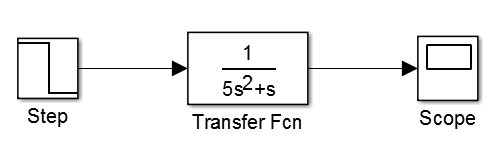
\includegraphics[scale=.5]{fq1.png}
    \caption{Sistema malha aberta}
    \label{fig:funcaoMalhaAberta}
\end{figure}

Para a entrada foi inserido os seguintes valores para o ''step'', \texttt{Step Time: 1e-3}, \texttt{Initial Value: 500}, \texttt{Final Value: 0}. A figura 
~\ref{fig:resultadoMalhaAberta} mostra o ângulo de saída da pá.

\begin{figure}[!ht]
	\centering
	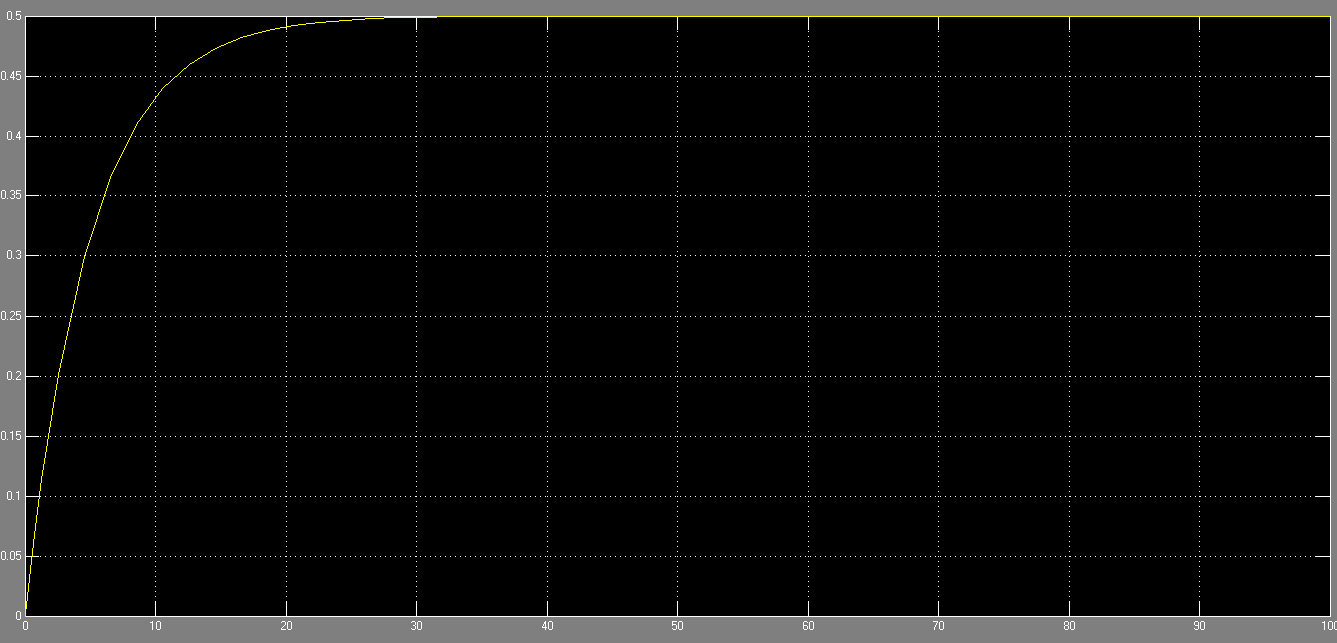
\includegraphics[scale=.3]{rq1.png}
    \caption{Resultado para o sistema malha aberta}
    \label{fig:resultadoMalhaAberta}
\end{figure}

\textbf{Comentários:} Nota-se facilmente que o ângulo obtido não era o esperado para o sistema. Efeito esse que poderia ser alterado ou corrigido com uma realimentação negativa do sistema. 

\section{Problema 2, a realimentação e o controlador proporcional}

Para este problema, foi inserido o controlador proporcional em série com a planta e uma realimentação negativa unitária. A entrada passa a ser não mais 
de 500 N/m e agora é considerando para efeitos fisicos um sinal de tensão.
A parametrização do valor do controlador proporcional foi feita de tal forma que o mesmo assuma os seguintes valores: 1, 5 e 10.

\begin{figure}[!ht]
	\centering
	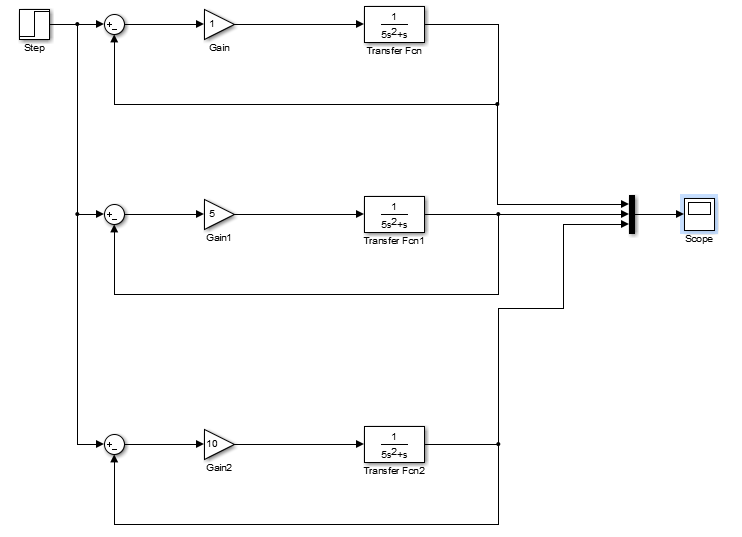
\includegraphics[scale=.6]{sq2.png}
    \caption{Modelo para o problema 2}
    \label{fig:modeloProblema2}
\end{figure}

A figura ~\ref{fig:modeloProblema2} mostra o modelo construido no simulink usando apenas um scope para a visualização do resultado. O step time foi configurando de tal maneira que os seus valores foram: \texttt{Step Time: 1}, \texttt{Initial Value: 1}, \texttt{Final Value: 0}.
O resultado para a simulação pode ser visualizado na figura ~\ref{fig:resultadoProblema2}

\begin{figure}[!ht]
	\centering
	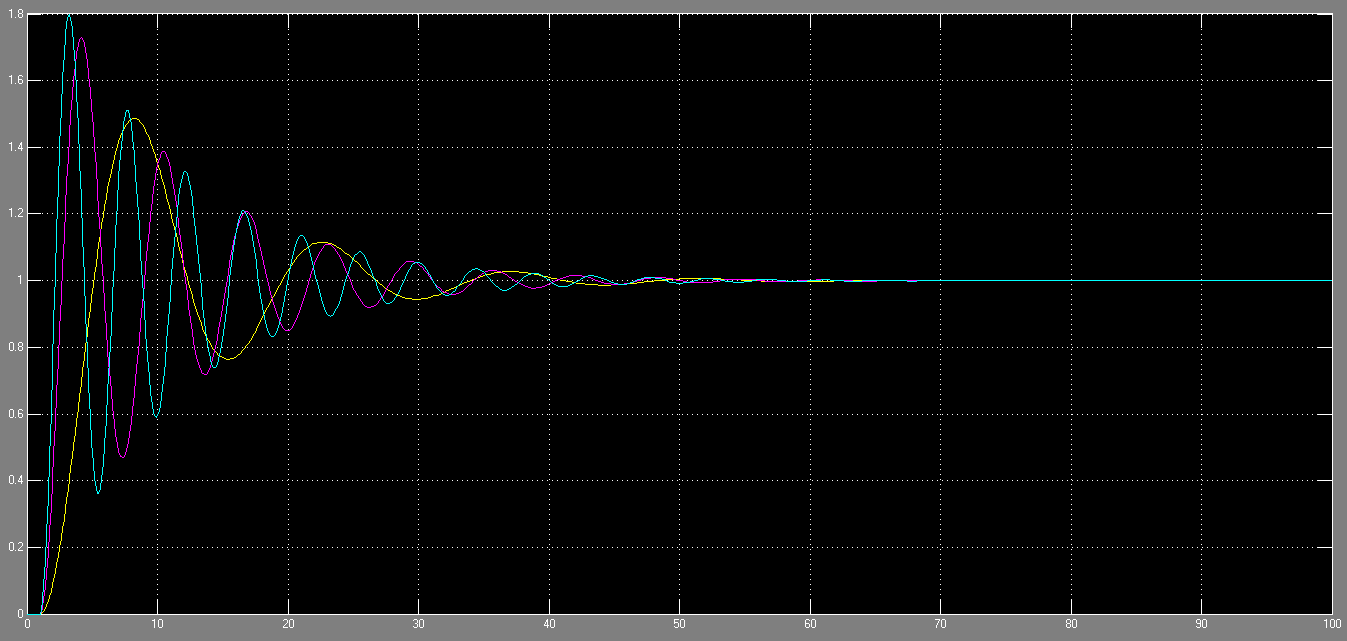
\includegraphics[scale=.3]{fq2.png}
    \caption{Resultado do problema 2}
    \label{fig:resultadoProblema2}
\end{figure}

O sistema agora se estabiliza no ponto desejado, em compensação temos a desagradavel situação dos oscilações no inicio. Oscilalções estas que podem
destruir a estrutura da pá, ou pior, todo o gerador éolico.

\section{Problema 3, a pertubação no sistema}

Para esta situação, temos uma pertubação no sistema, pertubação esta que pode ser proveniente de uma grande rajada de vento ou terremoto. O estudo da planta
e como ela se comporta para tal evento é feito da seguinte maneira. Um sinal
de 0.3 é inserido antes da planta e depois do controlador proporcional. Sinal este que não representa algo especifico, é utilizado apenas para efeitos matemáticos do problema. 
O resultado obtido para as 3 situações pode ser visto na figura ~\ref{fig:resultadoProblema3}.

\begin{figure}[!ht]
	\centering
	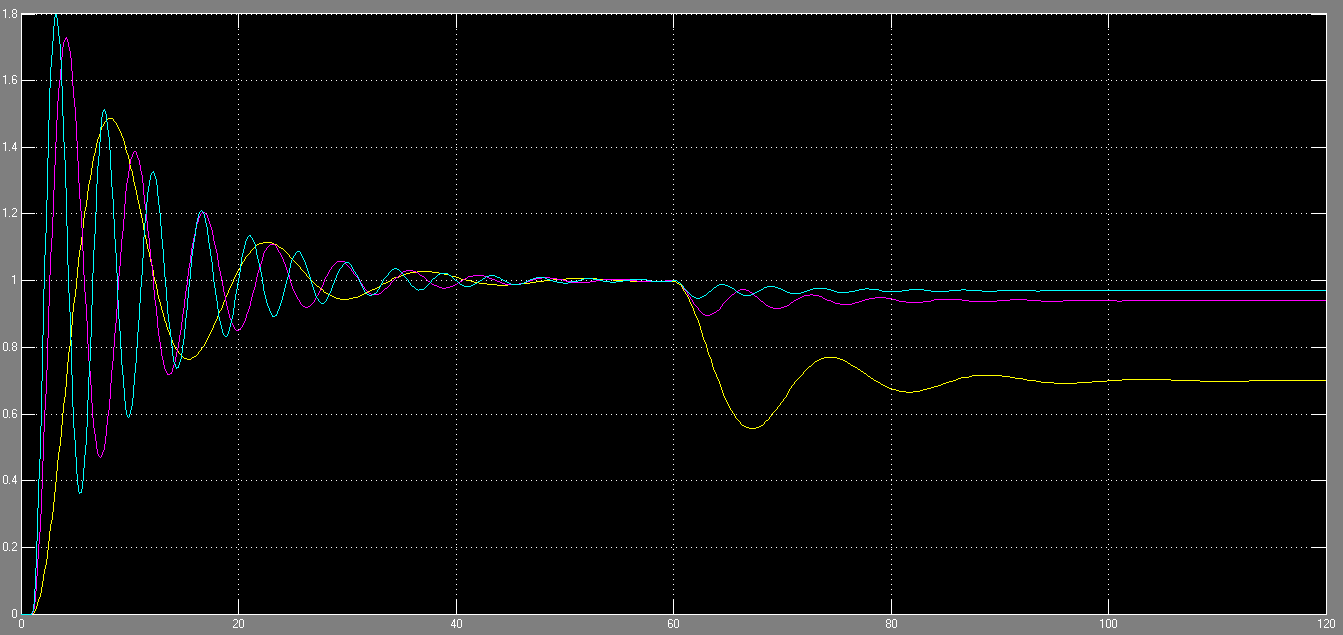
\includegraphics[scale=.3]{rq3.png}
    \caption{Resultado do problema 3}
    \label{fig:resultadoProblema3}
\end{figure}

No tempo 60 segundos após o inicio do processo o sinal de pertubação é inserido 
na planta, pode ser visto que o ângulo da pá é alterado e tal alteração é mantida.

\section{Problema 4, corrigindo com o integrador}

A tentativa agora é colocando um integrador antes da planta e da pertubação. O modelo do simulink é mostrado na figura ~\ref{fig:modeloIntregrador}

\begin{figure}[!ht]
	\centering
	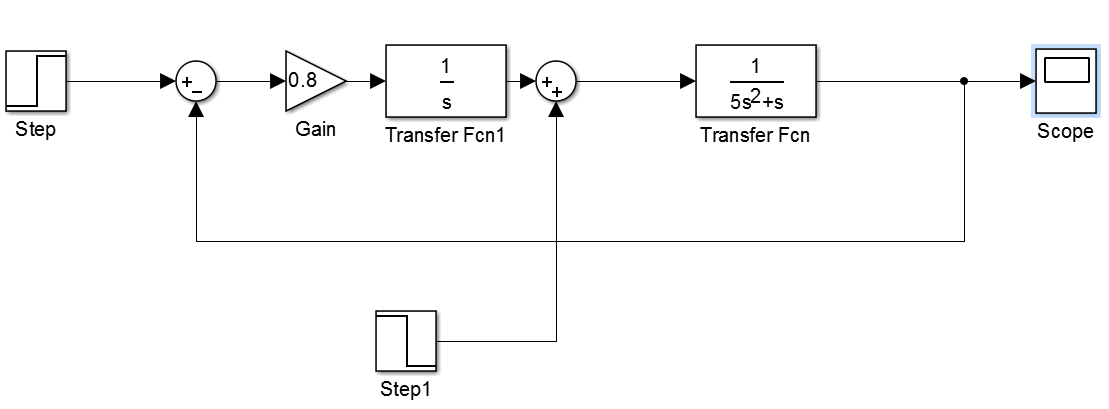
\includegraphics[scale=.3]{fq4.png}
    \caption{Modelo com o integrador}
    \label{fig:modeloIntregrador}
\end{figure}

O resultado para o efeito do integrador é mostrado na figura ~\ref{fig:respInstavelIntegrador}

\begin{figure}[!ht]
	\centering
	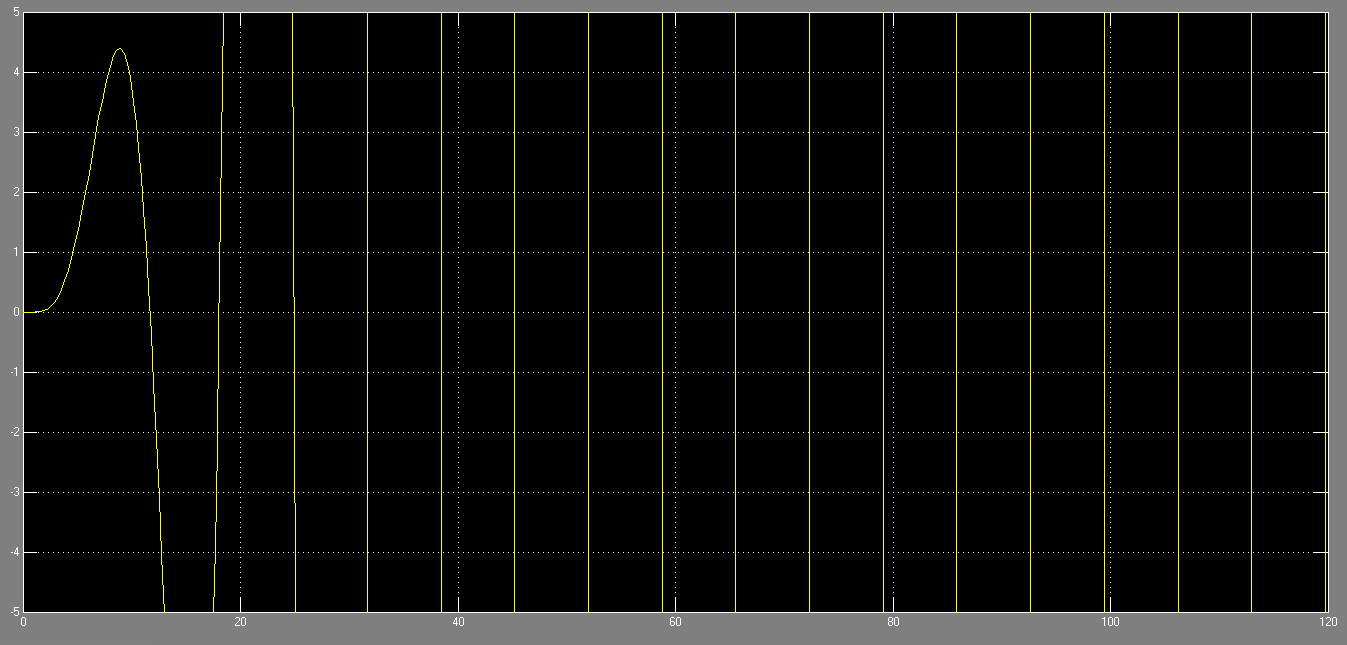
\includegraphics[scale=.3]{rq4.png}
    \caption{Resposta instável para o integrador}
    \label{fig:respInstavelIntegrador}
\end{figure}

Nota-se facilmente para a figura ~\ref{fig:respInstavelIntegrador} que o sistema é instável e não deve ser utilizado em nenhuma situação real.
O critério de estabilidade pode ser comprovado usando ''Routh'', aplicando
na equação de transferência,

\begin{equation}
\frac{\Theta(s)}{T_i(s)} = \frac{0.8}{5 s^3 + s^2 + 0.8}
\end{equation}

O critério de estabilidade fica,

\begin{center}
    \begin{tabular}{c| c c}
        $s^3$ & 5 & 0 \\
        $s^2$ & 1 & 8 \\
        $s^1$ & -4 & 0 \\
        $s^0$ & 0.8 & 0 \\
    \end{tabular}
\end{center}

\section{Problema 5, integrador}

O modelo para o integrador foi usando e ficou como mostra a figura ~\ref{fig:modint},

\begin{figure}[!ht]
	\centering
	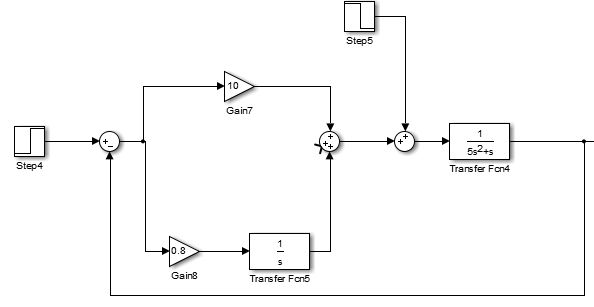
\includegraphics[scale=.5]{mqq5.png}
    \caption{Modelo para o integrador.}
    \label{fig:modint}
\end{figure}

O resultado é mostrado na figura ~\ref{fig:resint}

\begin{figure}[!ht]
	\centering
	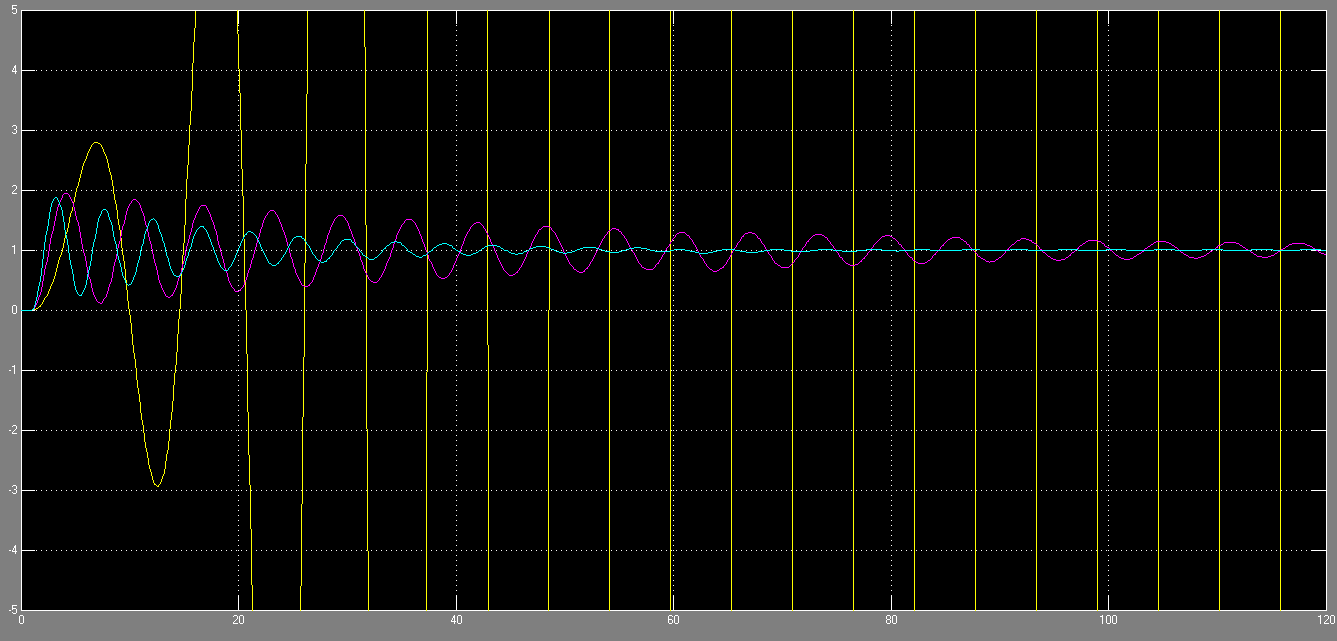
\includegraphics[scale=.3]{rqq5.png}
    \caption{Resposta integrador.}
    \label{fig:resint}
\end{figure}

Nota-se que o integrador corrigo o erro em regime permanente, entretanto
não é capaz de corrigir a estabilidade do sistema.

\section{Problema 6, derivador}

O modelo pode ser visto na figura

\begin{figure}[!ht]
	\centering
	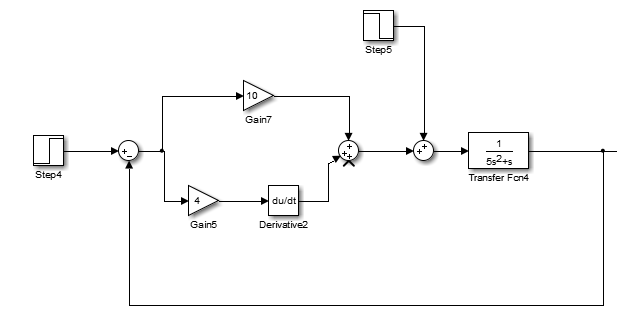
\includegraphics[scale=.5]{mq6.png}
    \caption{Modelo para o derivador.}
    \label{fig:modProb6}
\end{figure}

A resposta obtida foi,

\begin{figure}[!ht]
	\centering
	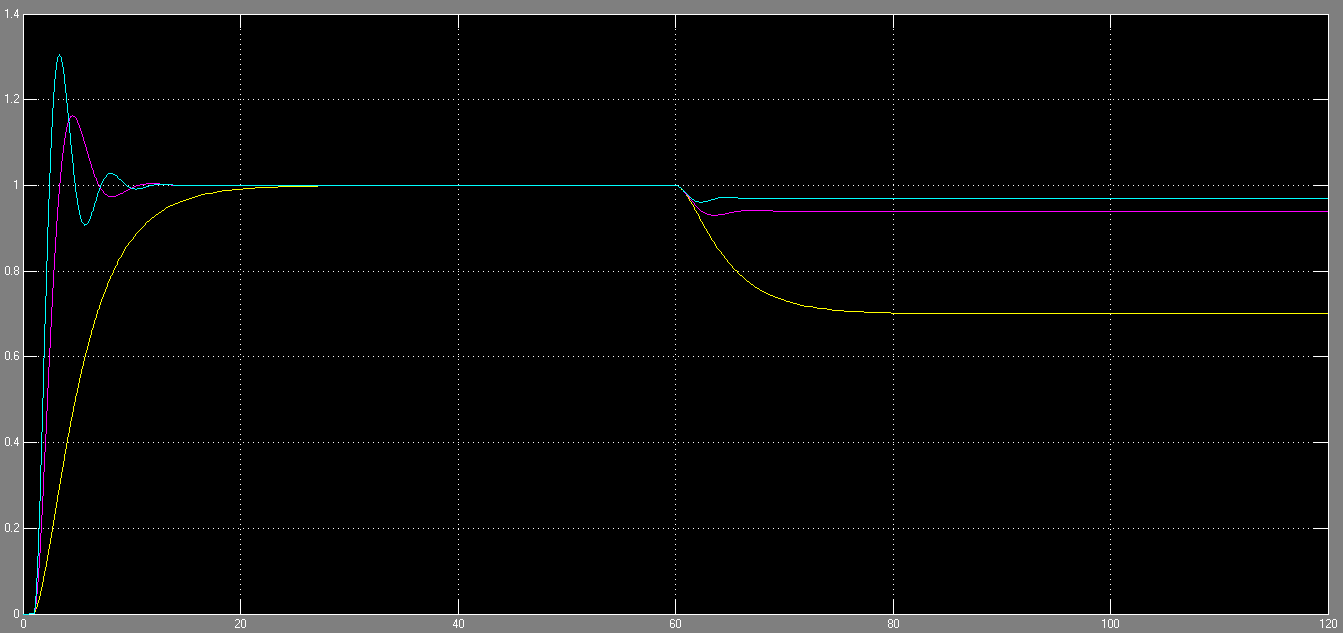
\includegraphics[scale=.3]{rq6.png}
    \caption{Resposta para o derivador.}
    \label{fig:resProb6}
\end{figure}

Nota-se que o derivador retira os efeitos de oscilação mas mantem 
o erro em regime permanente.

\section{Problema 7, Controle PID}

O controle PID completo foi usando e para tal a modelo no simulink é mostrado ~\ref{fig:modProb5}.

\begin{figure}[!ht]
	\centering
	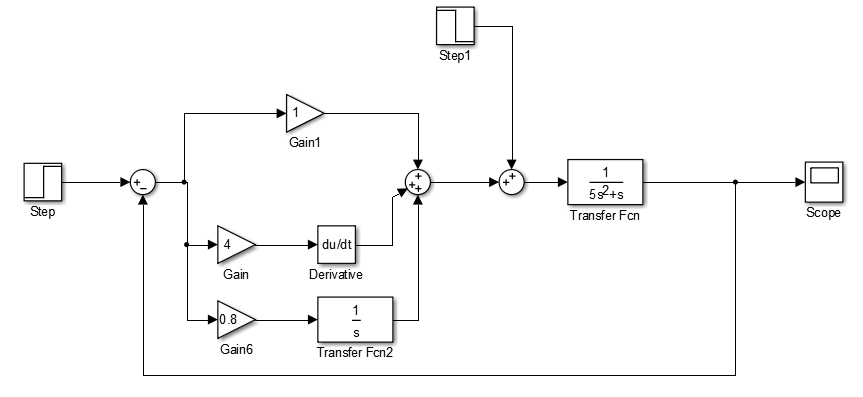
\includegraphics[scale=.5]{mq5.png}
    \caption{Modelo para o PID.}
    \label{fig:modProb5}
\end{figure}

A simulação parametrica para o problema, com o valor do ganho
propocional de 1, 5 e 10. O resultado pode ser visto na figura ~\ref{fig:resProb5}. 

\begin{figure}[!ht]
	\centering
	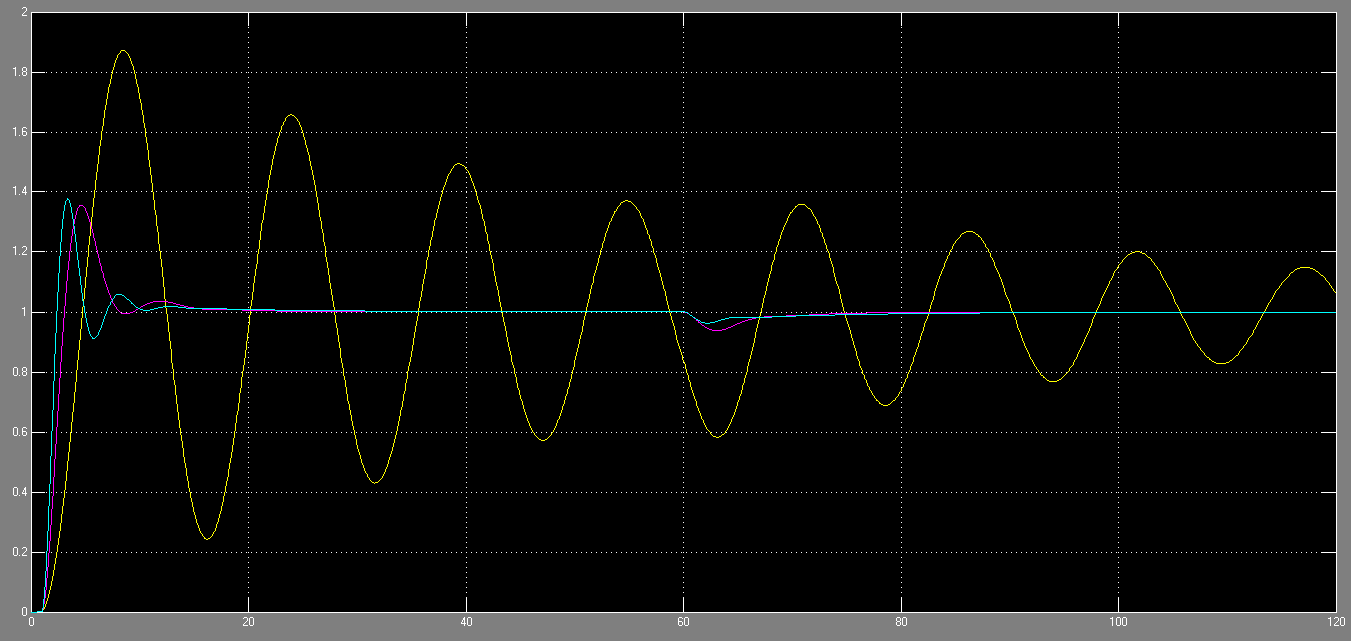
\includegraphics[scale=.3]{rq5.png}
    \caption{Resposta para o PID}
    \label{fig:resProb5}
\end{figure}

\end{document}